\documentclass{article}

% Language setting
\usepackage[english]{babel}

% Set page size and margins
% Replace `letterpaper' with `a4paper' for UK/EU standard size
\usepackage[letterpaper,top=2cm,bottom=2cm,left=3cm,right=3cm,marginparwidth=1.75cm]{geometry}

% Useful packages
\usepackage{amsmath}
% --- Code listings ---
\usepackage{listings}
\usepackage{xcolor}
\definecolor{codegreen}{rgb}{0,0.6,0}
\definecolor{codegray}{rgb}{0.5,0.5,0.5}
\definecolor{codepurple}{rgb}{0.58,0,0.82}
\definecolor{backcolour}{rgb}{0.95,0.95,0.92}

\lstdefinestyle{mystyle}{
    backgroundcolor=\color{backcolour},   
    commentstyle=\color{codegreen},
    keywordstyle=\color{magenta},
    numberstyle=\tiny\color{codegray},
    stringstyle=\color{codepurple},
    basicstyle=\ttfamily\footnotesize,
    breakatwhitespace=false,         
    breaklines=true,                 
    captionpos=b,                    
    keepspaces=true,                 
    numbers=left,                    
    numbersep=5pt,                  
    showspaces=false,                
    showstringspaces=false,
    showtabs=false,                  
    tabsize=2
}

\lstset{style=mystyle}
% --- End Code Listings
\usepackage{graphicx}
\usepackage{float}
\usepackage{caption}
% \captionsetup{labelformat=empty} 
% \usepackage{subcaption}
\usepackage[colorlinks=true, allcolors=blue]{hyperref}
\graphicspath{{./figures/}}

\title{ECE 637 Lab - Image Halftoning}
\author{Colin Braun}

\begin{document}
\maketitle

\section{Thresholding and Random Noise Binarization}
\subsection{Original image and result of thresholding}
\begin{figure}[H]
    \centering
    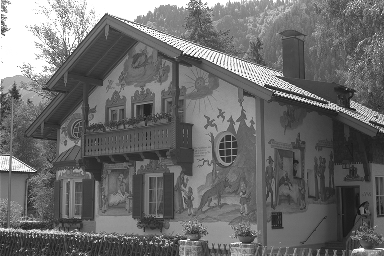
\includegraphics[width=1\textwidth]{../house.png}
    \caption{Original image.}
\end{figure}
\begin{figure}[H]
    \centering
    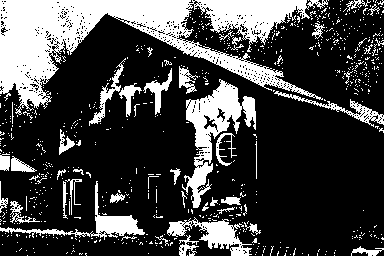
\includegraphics[width=1\textwidth]{../3-thresholded-image.png}
    \caption{BW image after applying threshold}
\end{figure}
\subsection{Computed RMSE and fidelity values}
\textbf{RMSE}: 10.03
\textbf{Fidelity}: 77.34
\subsection{Code for fidelity function}
\lstinputlisting[language=Python, firstline=18, lastline=37]{../section3.py}

\section{Ordered Dithering}
\subsection{The three Bayer index matrices of sizes 2 × 2, 4 × 4, and 8 × 8}
\begin{figure}[H]
    \begin{equation*}
        \begin{bmatrix}
        1 & 2\\
        3 & 0\\
        \end{bmatrix}
    \end{equation*}
\caption{2x2 Bayer index matrix.}
\end{figure}
\begin{figure}[H]
    \begin{equation*}
        \begin{bmatrix}
        5 & 9 & 6 & 10\\
        13 & 1 & 14 & 2\\
        7 & 11 & 4 & 8\\
        15 & 3 & 12 & 0\\
        \end{bmatrix}
    \end{equation*}
\caption{4x4 Bayer index matrix.}
\end{figure}
\begin{figure}[H]
    \begin{equation*}
        \begin{bmatrix}
        21 & 37 & 25 & 41 & 22 & 38 & 26 & 42\\
        53 & 5 & 57 & 9 & 54 & 6 & 58 & 10\\
        29 & 45 & 17 & 33 & 30 & 46 & 18 & 34\\
        61 & 13 & 49 & 1 & 62 & 14 & 50 & 2\\
        23 & 39 & 27 & 43 & 20 & 36 & 24 & 40\\
        55 & 7 & 59 & 11 & 52 & 4 & 56 & 8\\
        31 & 47 & 19 & 35 & 28 & 44 & 16 & 32\\
        63 & 15 & 51 & 3 & 60 & 12 & 48 & 0\\
        \end{bmatrix}
    \end{equation*}
\caption{8x8 Bayer index matrix.}
\end{figure}
\subsection{The three halftoned images produced by the three dither patterns}
\begin{figure}[H]
    \centering
    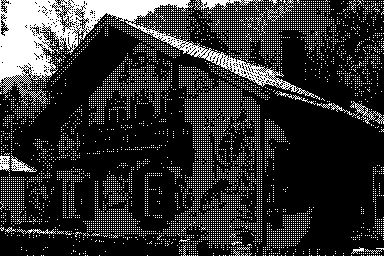
\includegraphics[width=1\textwidth]{../4-b2x2.png}
    \caption{Result using 2x2 index matrix.}
\end{figure}
\begin{figure}[H]
    \centering
    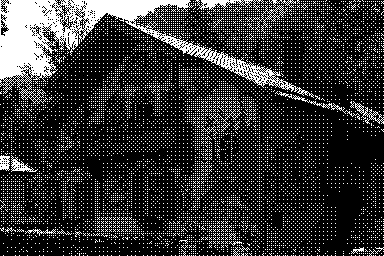
\includegraphics[width=1\textwidth]{../4-b4x4.png}
    \caption{Result using 4x4 index matrix.}
\end{figure}
\begin{figure}[H]
    \centering
    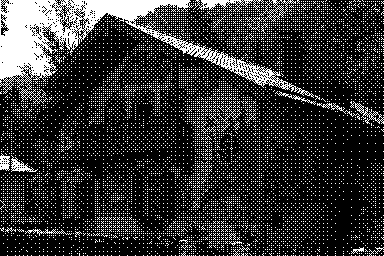
\includegraphics[width=1\textwidth]{../4-b8x8.png}
    \caption{Result using 8x8 index matrix.}
\end{figure}
\subsection{The RMSE and fidelity for each of the three halftoned images}
\begin{center}
    \begin{tabular}{|c|c|c|}
        \hline
        Matrix Size & RMSE & Fidelity \\
        \hline
        2x2 & 97.67 & 50.06 \\
        \hline
        4x4 & 101.01 & 16.56 \\
        \hline
        8x8 & 100.91 & 14.69 \\
        \hline
    \end{tabular}
\end{center}

\section{Error Diffusion}
\subsection{Error diffusion Python code}
\lstinputlisting[language=Python]{../section5.py}
\subsection{Error diffusion result}
\begin{figure}[H]
    \centering
    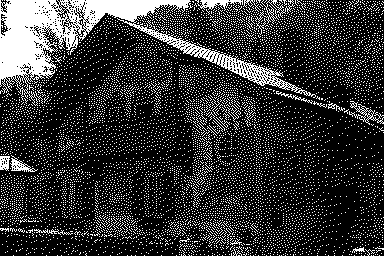
\includegraphics[width=1\textwidth]{../5-diffusion-result.png}
    \caption{The error diffusion result}
\end{figure}
\subsection{The RMSE and fidelity of the error diffusion result}
\textbf{RMSE}: 99.15
\textbf{Fidelity}: 11.66
\subsection{Tabulated RMSE and fidelity results}
\begin{center}
    \begin{tabular}{|c|c|c|}
        \hline
        \textbf{Method} & \textbf{RMSE} & \textbf{Fidelity} \\
        \hline
        Simple Thresholding & 10.03 & 77.33 \\
        \hline
        Ordered Dithering (2x2) & 97.67 & 50.06 \\
        \hline
        Ordered Dithering (4x4) & 101.01 & 16.56 \\
        \hline
        Ordered Dithering (8x8) & 100.91 & 14.69 \\
        \hline
        Error Diffusion & 99.15 & 11.66 \\
        \hline
    \end{tabular}
\end{center}
It might seem surprising that simple thresholding produces the least RMSE in a convincing manner. However, this is to be expected, since choosing either black or white depending on which one the original pixel is closer to will make this error as small as possible. Of course, when smoothing is applied to compute the fidelity, the results are not quite ideal. The other methods are designed with the intent that the smoothed result will be closer to the original image, resulting in substantially better fidelity. Among these methods, the ordered dithering (2x2) case be both qualitatively and quantitatively seen to have low fidelity. This case has such large jumps between index values/thresholds of the matrix that we do not get black and white pixels distibuted in a way that would result in an image of higher fidelity when it is smoothed. In general, the non- simple thresholding methods are not concerned about the RMSE, but instead focus on the visual quality when the image is smoothed.

\end{document}
